\subsubsection{$\textrm{PM}_{2.5}$ Monitor data from US EPA AQS Air Data Query Tool}

\subsubsection*{To Do}
\begin{enumerate}
	\item Download the 2018 data again - the complete 2018 data should be available by July 2019.
\end{enumerate}

\subsubsection*{Data Source}

\begin{itemize}[nolistsep]
\item \textbf{Contact} Can email the Air Quality Analysis Group (U.S. EPA Office of Air Quality Planning and Standards) on their website at \url{https://www.epa.gov/outdoor-air-quality-data/forms/contact-us-about-outdoor-air-quality-data}


\item \textbf{Citation/Link}

United States Environmental Protection Agency. \textit{Pre-Generated Data Files: Daily Summary Files, PM2.5 FRM/FEM Mass (88101) and PM2.5 non FRM/FEM Mass (88502), 2008-2018}. \url{https://aqs.epa.gov/aqsweb/airdata/download_files.html#Daily}.  Download spreadsheet listing all AQS monitors with datums (\url{https://aqs.epa.gov/aqsweb/airdata/aqs_monitors.zip}) from ``Monitor Listing" at \url{https://aqs.epa.gov/aqsweb/airdata/download_files.html#Meta}. The file name is aqs\_monitors.csv in the AQS\_Daily\_Summaries folder in the S3 data.
\item \textbf{Data (local)}
\item \textbf{Geographic Extent}
\item \textbf{Temporal Extent}
2008 through 2018. The 2018 file was downloaded June 14, 2019, and it is possible that more 2018 data will become available after this date.
\item \textbf{Acknowledgment} EPA
\end{itemize}



\subsubsection*{Brief Description}

We downloaded PM\textsubscript{2.5} data from both the US EPA AQS Air Data Query Tool \citep{EPAAirData2017}  for the 11-state region (Figure \ref{fig:Map11States}) including any of the following parameter codes: 88101, 88500, 88502, 81104 \citep{EPANPM25Memo2017,EPANPM25Parameters2017,EPANAllParameters2017}. 

%\subsubsection*{Notes}

%\subsubsection*{File Format}

%\subsubsection*{Data Filtering and Processing}

%\subsubsection*{Final Variable(s)}

%\subsubsection*{Methods}

%\subsubsection*{Quality Control}

\subsubsection*{Data File Names}

\begin{enumerate}[noitemsep]
\item daily\_88101\_2008.csv
\item daily\_88101\_2009.csv
\item daily\_88101\_2010.csv
\item daily\_88101\_2011.csv
\item daily\_88101\_2012.csv
\item daily\_88101\_2013.csv
\item daily\_88101\_2014.csv
\item daily\_88101\_2015.csv
\item daily\_88101\_2016.csv
\item daily\_88101\_2017.csv
\item daily\_88101\_2018.csv * this is only part of 2018 - the rest will need to be downloaded once it becomes available
\item daily\_88502\_2008.csv
\item daily\_88502\_2009.csv
\item daily\_88502\_2010.csv
\item daily\_88502\_2011.csv
\item daily\_88502\_2012.csv
\item daily\_88502\_2013.csv
\item daily\_88502\_2014.csv
\item daily\_88502\_2015.csv
\item daily\_88502\_2016.csv
\item daily\_88502\_2017.csv
\item daily\_88502\_2018.csv * this is only part of 2018 - the rest will need to be downloaded once it becomes available
\end{enumerate} 

%\begin{figure}[H] % start figure float, this method seems to have fewer options for location specifier, H, t, c, and b should work
%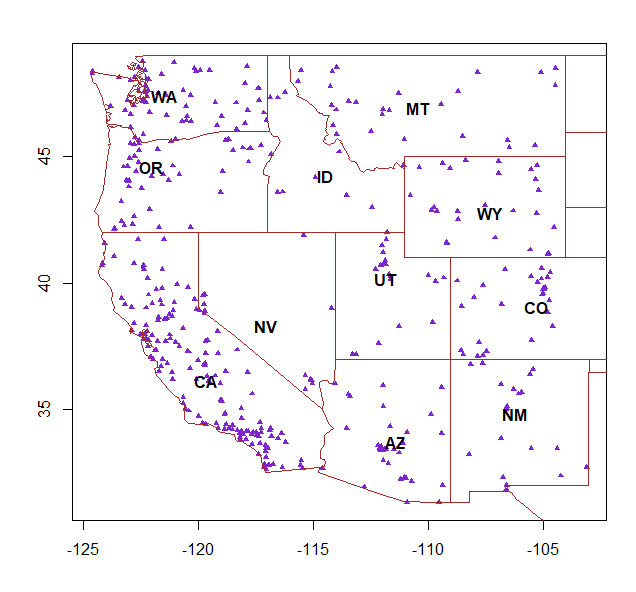
\includegraphics[width=1\textwidth]{m88101and88502notitlenorlabels.PNG} %
%\caption{\label{fig:MapLocations}Map of 88101 and 88502 PM\textsubscript{2.5} Monitors.} % The text after \label{} is what shows up as the caption. Inside the brackets for \label{} is just for linking figures to text and is analogous to the AuthorYear in citations. 
%\end{figure} % end figure float

\subsubsection*{Script Names}

\begin{enumerate}
\item process\_PM25\_EPA\_data\_source\_function.R (called from Process\_PM25\_data\_step1.R)
\end{enumerate}
